\chapter{Background}
\label{Chapter2}
The two computationally intense algorithms, highlighted in this report involve an encryption algorithm and a neural network.Analyzing the underlying arithmetic require a detailed knowledge of the underlying concepts and basis of the algorithm. A thorough understanding of the operations and number representations specific to the arithmetic is also a prerequisite to manipulate an algorithm's underlying mathematics. In this chapter the basics of encryption algorithm, neural networks, number representations and fixed point mathematics is discussed in detail.
\section{Cryptography}
Cryptography was invented with an intent of secure communication.It prevents unauthorized users to access and modify the data, ensuring reliable communication by avoiding data corruption and also helps prevent in information loss. Various applications involving cryptography include military applications, smart cards, passwords etc.

\noindent Two main processes involved in cryptography are encryption and decryption:
\vspace{0.25cm}
\begin{itemize}
\label{Encryption}
\item
\textbf{Encryption} is a process of converting the data in a complicated form such that it is not readable by unintended users. Encryption is performed on a data known as plaintext to generate another form of data which is encrypted known as ciphertext.

\item
\label{Decryption}
\vspace{0.25cm}
\textbf{Decryption} is a process of converting the data in a readable form from an unintelligible form only by the intended users.
\end{itemize}

\noindent Modern cryptographical algorithms are based on computationally hard mathematical operations and computer science practices, and hence the require faster computing technology for efficiency.

\noindent Encryption is of two types:
\begin{enumerate}
\item
\textbf{Symmetric Encryption:} In this type of encryption, a single key is used for encryption as well as decryption.
\item
\textbf{Asymmetric Encryption:} In this type of encryption scheme two different keys are used, public key is used to encrypt a piece of information and a secret key is used for decryption. The public key is usually available publicly, whereas the secret key is only provided to the intended users. Asymmetric encryption is more computationally intense as compared to symmetric encryption and hence requires more processing power and at times is slower. 
\begin{figure}[!h]
\centering
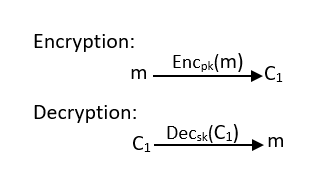
\includegraphics[scale=0.8]{figures/asym.PNG}
\caption{Asymmetric Encryption and Decryption}
\label{fig:Asymmetric Encryption}
\end{figure}

\end{enumerate}
With the advancement of cloud based applications which at times deal with sensitive information require data to be encrypted prior to storing it to cloud. Homomorphic encryption is devised to use the computational power of cloud.
\subsection{Homomorphic Encryption}
The basic idea of homomorphic encryption scheme is to delegate the processing of data to the cloud without giving access to it.

\vspace{0.25cm}
\noindent Let us say a user has  a set of confidential data and he or she wants to process that data on a cloud or server. The normal procedure would be as specified in the figure \ref{fig:Conventional Encryption} wherein the user encrypts the data to be processed and send it to server. At the server end, the data is decrypted using the secret key, the computation is performed and the resulting data is again encrypted and sent back to the user, which the user can decrypt to get back the end result of the computation.
%figure

\begin{figure}[!h]
\centering
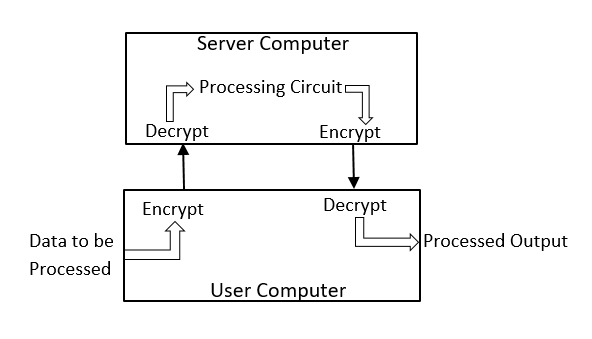
\includegraphics[scale=0.7]{figures/Capture1.PNG}
\caption{Conventional Encryption}
\label{fig:Conventional Encryption}
\end{figure}
%http://www.americanscientist.org/libraries/documents/201286159329266-2012-09CompSciHayes.pdf
\vspace{0.25cm}
However if the user want a secure application, wherein the data is not decrypted even at server, homomorphic encryption is used. It allows performing computations over encrypted data, resulting in a data which when decrypted gives back the original result after performing the computation on plain text (Refer figure \ref{fig:Homomorphic Encryption}).
%figure 

\begin{figure}[H]
\centering
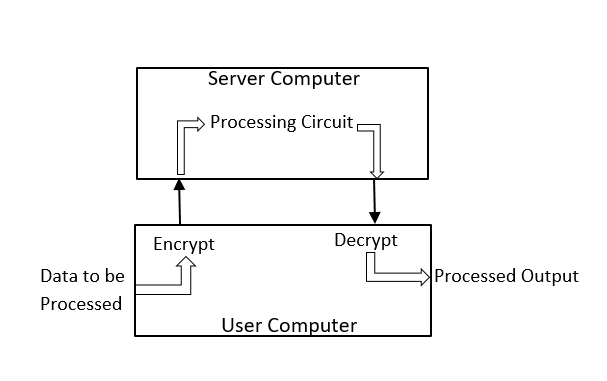
\includegraphics[scale=0.7]{figures/Capture.PNG}
\caption{Homomorphic Encryption}
\label{fig:Homomorphic Encryption}
\end{figure}
\subsubsection{Steps involved in Homomorphic Encryption} \label{steps}
Typically any encryption scheme involves three algorithms,
\begin{enumerate}
    \item 
    \textbf{Keygen:} Here in a L bit-length key is generated using an algorithm. In case of symmetric encryption schemes, a single key is generated for both encryption and decryption. In case of Asymmetric encryption scheme, two keys are generated: Public key(pk) which is available to all users and is used for encryption of message and a Secret key(sk) which is used for decryption and is available only to the intended users.
   \item
    \textbf{Encryption:} As specified in \ref{Encryption} encryption is a process of encoding a message using a key to form a ciphertext.
    \item
    \textbf{Decryption:} As specified in \ref{Decryption} decryption is a process of decoding a ciphertext back to original readable form using a key.
   
   \noindent A homomorphic encryption has an additional algorithm involved in addition to the above three.
    \item 
     \textbf{Evaluate:} Evaluate is associated with a set of functions, for which the computation is supported by the scheme. A function f on a set of numbers (n\textsubscript{1},n\textsubscript{2},......,n\textsubscript{t}) is intended to be performed, where (c\textsubscript{1},c\textsubscript{2},......,c\textsubscript{t}) represent the encryption of given numbers using a public key(pk),under the homomorphic encryption scheme.The result of evaluate algorithm 'c' which is applied on (c\textsubscript{1},c\textsubscript{2},......,c\textsubscript{t}) to perform the function f is the encryption of f(n\textsubscript{1},n\textsubscript{2},......,n\textsubscript{t}) under the public Key(pk). In other words, if we decrypt the result of evaluate algorithm with the corresponding secret key we get back f(n\textsubscript{1},n\textsubscript{2},......,n\textsubscript{t}).
     
     \noindent The efficiency of evaluation function depends primarily on the size of ciphertexts and the function being computed.
     \end{enumerate}
     The above works only for a set of functions which are allowed or supported by the encryption scheme. 
    
\subsubsection{Issues with Homomorphic Encryption Scheme} \label{limitations}
\begin{itemize}
\item
\textbf{Semantic Security:} Semantic security refers to the security in terms of the one wayness of encryption algorithm. i.e. There should not be any polynomial time algorithm which can guess the plaintext and private key(pk). To ensure semantic security an encryption scheme must present multiple encryptions for the same plaintext given a public key. However if there is always a one to one mapping,the scheme can not be ensured to be secure. So encryption algorithms should be hard enough to be broken by attackers. 
\item 
\textbf{Noise in Ciphertexts:} When a ciphertext is encrypted, a fixed term is added to it to ensure the security of the scheme which is called noise. It may be a small number or some polynomial based on whether the scheme is for integers or polynomials.A ciphertext can be decrypted if and only if the noise is less than a certain maximum value. As certain operations are performed on the ciphertexts in homomorphic encryption, the noise grows. The increase in noise in the final ciphertext is based on the operation and also on the depth of operations.

 \noindent Given the encryption function as $Enc(x)=a\times r+b\times n+x$ where x is the message, r is a random variable, a is the secret key, n is the noise.The decryption can be performed on the above encryption function as: 

 \noindent\hspace{3cm} $Dec(Enc(x))=Enc(x)-(a\bmod q)\times r$
 
 \noindent i.e.\hspace{2.7cm}$Dec(Enc(x))= b\times n+x$
 
 \noindent and x can be computed from the above as:
 
 \noindent\hspace{3cm} $x=(b\times n+x)\bmod b$

\vspace{0.25cm}
 \noindent Consider two ciphertexts c\textsubscript{1} and c\textsubscript{2} which are the encryptions of m\textsubscript{1} and m\textsubscript{2} after addition of noise n\textsubscript{1} and n\textsubscript{2}, such that
 
 \noindent\hspace{3cm} $c\textsubscript{1}=a\times r\textsubscript{1}+b\times n\textsubscript{1}  +m\textsubscript{1}$
 
 and 
 
 \noindent\hspace{3cm}$c\textsubscript{2}=a\times r\textsubscript{2}+b\times n\textsubscript{2}  +m\textsubscript{2}$
 
 \noindent Addition Operation on the ciphertexts, will result in a new ciphertext c\textsubscript{3} which can be given as:

 \noindent\hspace{3cm} $c\textsubscript{3}=c\textsubscript{1}+c\textsubscript{2}$
 
 \noindent\hspace{3cm} $c\textsubscript{3}=a\times (r\textsubscript{1}+r\textsubscript{2})+b\times (n\textsubscript{1}+n\textsubscript{2}) +(m\textsubscript{1}+m\textsubscript{2})$  \hfill                                                                   eq[2.1]

 \noindent From equation eq[2.1] it can be seen that 
\begin{itemize}
\item
 \noindent $r\textsubscript{3}=r\textsubscript{1}+r\textsubscript{2}$
\item
 \noindent $m\textsubscript{3}= r\textsubscript{1}+ r\textsubscript{2}$

\vspace{0.25cm}
 \noindent The decryption of the result can be performed as:

 \noindent\hspace{3cm} $Dec(c\textsubscript{3})=c\textsubscript{3}-(a\bmod q)\times r\textsubscript{3}$
 
 \noindent hence,\hspace{2cm}$Dec(c\textsubscript{3})=b\times (n\textsubscript{1}+n\textsubscript{2}) +(m\textsubscript{1}+m\textsubscript{2})$
\item
The noise after addition is the  addition of noise of individual cipher texts. i.e. 
$n\textsubscript{3}=(n\textsubscript{1}+n\textsubscript{2})$
\end{itemize}

 \noindent Similarly multiplication operation on the cipher texts, will result in a new ciphertext c\textsubscript{3} which can be given as:
 
$c\textsubscript{3}=c\textsubscript{1}\times c\textsubscript{2}$

$c\textsubscript{3}=(a\times r\textsubscript{1}+b\times n\textsubscript{1} +m\textsubscript{1})\times (a\times r\textsubscript{2}+b\times n\textsubscript{2}  +m\textsubscript{2})$

$c\textsubscript{3}=(a^{2}\times r\textsubscript{1}\times r\textsubscript{2})+(a\times b\times r\textsubscript{1}\times n\textsubscript{2})+(a\times r\textsubscript{1}\times m\textsubscript{2})+(b\times a\times n\textsubscript{1}\times r\textsubscript{2})+(b^{2}\times n\textsubscript{1}\times n\textsubscript{2})
+(b\times n\textsubscript{1}\times m\textsubscript{2})+(m\textsubscript{1}\times a\times r\textsubscript{2})+(m\textsubscript{1}\times b\times n\textsubscript{2})+(m\textsubscript{1}\times m\textsubscript{2})$         \hfill                                        eq[2.2]

From equation eq[2.2] it can be seen that
\begin{itemize}
\item
 \noindent $r\textsubscript{3}=r\textsubscript{1}\times r\textsubscript{2}$
\item
The noise after multiplication is approximately the product of noise of individual cipher texts. i.e.
$n\textsubscript{3}=(n\textsubscript{1}\times n\textsubscript{2})$
\end{itemize}
Hence the resulting cipher text after performing computation has more noise than the input cipher texts. Also multiplication operation  tends  to  increase  the noise faster(by squaring the noise) than addition or subtraction which result in addition of noise. Usually cipher texts generated after the result of operation, will require more bits for noise, than the input cipher texts. e.g. for multiplication double the number of bits are required to store the resulting noise which is the multiplication of individual noises.
\item
\textbf{Number of Output Bits:} After performing the computation, it may happen that the output may have lesser or more number of bits then the original message. But from hardware point of view the number of output pins is fixed, so the output generated by the encryption may be either truncated or zero padded, based on the number of output bits. So it is difficult to know in prior, the exact number of bits in the output, while executing a function on cloud.

\end{itemize}

 \subsection{Somewhat Homomorphic Encryption Scheme}
     Usually the complexity of a scheme depends on the function being computed. At times the run-time evaluation can be measured based on the time taken to execute the same function on a turing machine. The function can be broken down into a set of AND, OR or NOT gates for circuit level representation. As these can be computed using addition, subtraction and multiplication, an encryption scheme that supports an indefinite number of addition, subtraction and multiplication operations is needed.
   
     \noindent But considering the limitations of homomorphic encryption scheme as referred in section \ref{limitations}, an indefinitely computing circuit might not be feasible because with repeated operations the noise grows and if the noise is too large it is difficult to decrypt the ciphertexts. So there is a limitation on the depth of the homomorphic encryption scheme. A scheme which allows the computation of a limited number of functions is called somewhat homomorphic encryption scheme. Such schemes allow the addition, subtraction and multiplication operations, to be performed only to a depth such that the noise in resulting ciphertext is below the maximum limit. 
 \subsection{Fully Homomorphic Encryption Scheme}  
 Fully Homomorphic Encryption Scheme allows to perform arbitrary computations on encrypted data. The number of operations and type of operation is not a restriction, as opposing to somewhat homomorphic encryption schemes. It works for all type of functions. FHE is more generalized but it is more computationally intense as compared to somewhat homomorphic schemes. A Fully Homomorphic scheme can be devised from a somewhat homomorphic scheme by using the process called bootstrapping.

 \vspace{0.25cm}
  \noindent \textbf{Bootstrapping:} Bootstrapping is referred to the self referential property of the encryption scheme such that it is able to perform its own decryption homomorphically, in addition to other operations e.g. addition , subtraction and multiplication. The evaluation function of such schemes are in such a way that it performs decryption of the secret key homomorphically, resulting in a new ciphertext, which has the noise component lower than the original ciphertext. In other words, it is a method to reset the noise level in ciphertexts. It results in the encryption of the original text under a different secret key. The process is also known as key switching. This scheme is feasible only if the decryption circuit or function is not complex. It is considered that the decryption is simpler for lattice based cryptosystems. 
  
\subsection{Levelled Fully Homomorphic Encryption scheme}
An Encryption scheme is said to be LFHE, if it uses the same decryption circuit for all the functions but the depth to which the functions will be computed is fixed and constant. The depth specifies the number of gates that can be used to implement a function. 

\section{Proposed FHE using Ideal Lattices} \label{FHE}
A scheme is proposed in [\ref{lattices}], for the implementation of a fully homomorphic encryption scheme. It is based on lattice based cryptosystems for ideal lattices, as lattice based cryptosystems provide simpler decryption circuits. The scheme proposed in the paper is a levelled fully homomorphic scheme.

 \noindent The scheme is based on an algorithm called \textit{Recrypt} which is described below:
 
\vspace{0.25cm} \label{refresh}
\noindent \textbf{Recrypt:} Given a ciphertext c\textsubscript{1} of a message m encrypted under the key pk\textsubscript{1}, and another ciphertext c\textsubscript{11} which is the encryption of c\textsubscript{1} with another public key pk\textsubscript{2}. Also sk\textsubscript{11} is given as the encryption of secret key sk\textsubscript{1} for the public key pk\textsubscript{1} under pk\textsubscript{2}. As per the above algorithm,
if the evaluation function that can perform the decryption homomorphically, computes


\hspace{3cm} Evaluate\{pk\textsubscript{2}, Decryption, c\textsubscript{11},sk\textsubscript{11}\},

 \noindent the output will be another ciphertext c\textsubscript{2}, which is the encryption of m with the public key pk\textsubscript{2}. 
 
 \noindent As per the algorithm, the error vector corresponding to the initial encryption is removed here, and a new noise is added corresponding to the second encryption key pk\textsubscript{2}. The scheme works if the newly introduced error vector is smaller than the first.

 \noindent If the circuit is a d depth circuit, the public keys and secret keys in such cases will be a vector with atleast d public keys, each corresponding to each gate. 
Hence the \textit{keygen} function as referenced in section \ref{steps} is modified such that it generates d number of public and secret keys.
The complexity of such a scheme is huge,as a number of encryptions and decryptions are applied all along the depth of the circuit.
\section{Neural Networks}
A neural network is a programming approach in which a computer learns from data. The data can be collected from observations. Neural networks solve the problems in the same way as human beings, with the usage of a large number of artificial unit called neurons. These days neural networks provides basis for a lot of machine learning algorithms e.g image processing algorithms, speech recognition algorithm etc.

 \noindent Typically neural networks have layers which are composed of multiple interconnected nodes. The input is presented in input layer, and the output generated in the output layer is the weighted sum of the inputs after processing through a number of hidden layers of the network, where the weights are defined by learning or training the system based on computational data, which involve several times back propagation of data and adjustment of weights.
\subsection{Shallow Neural Networks} 
Shallow neural networks have only one hidden layer between input and output layer. Shallow networks are mostly for supporting vector machines or to map one function as a lookup table.
\subsection{Deep Neural Networks} Deep Neural networks have several hidden layers between the input and output layers. Deep neural networks represent complex functions with smaller number of units and weights, and also allow for reuse of results of one computation if the computation supports parallel computing. The details of the various layers used in the current implementation is described in Chapter \ref{Chapter4}.

\section{Floating Point Vs Fixed Point Representation}
 In floating point notation numbers are represented in 32-bit format,where 23-bits are used to store fraction and 8 bits are used to store the exponent and 1 bit stores the sign of the number e.g. IEEE 754 standard to represent 32-bit floating point number:

The number represented in the figure \ref{fig:Float Representation} is 0.15625, which can be calculated as:

\vspace{0.25cm}
\hspace{3cm}
$Number= (-1)^{sign}\times (1\times b\textsubscript{-1}b\textsubscript{-2}....b\textsubscript{-23})\textsubscript{2}\times 2^{(e-127)}$  

\vspace{0.25cm}
\noindent Specific decoders are needed to access the floating point numbers stored in memory on hardware, as floating numbers have a variable exponent which leads to a wide range of numbers which is non linear. Floating point numbers require resources e.g. address buses of 32 bits length.

\vspace{0.25cm}
\noindent In fixed point notation the numbers are represented with minimum 16 bits usually and the position of binary point is fixed so locating the decimal point is easy.
\begin{figure}[!h]
\centering
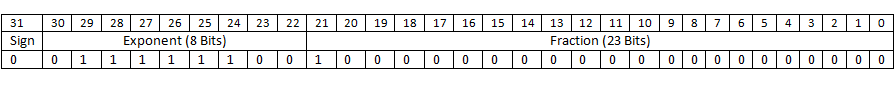
\includegraphics[scale=0.65]{figures/float.PNG}
\caption{Floating Point Number Representation}
\label{fig:Float Representation}
\end{figure}
\vspace{0.25cm}
 \noindent In Hardware, it is easy to store integers. e.g. an unsigned short integer in C will be represented as a 16 bit register in hardware. Even various arithmetic operations on integer numbers can be easily mapped to hardware e.g. addition of two unsigned short integers can be mapped as 16 1-bit additions. On heterogeneous platforms e.g. FPGA, Fixed point mathematical operations are performed in the same manner as integer mathematical operations. It uses lesser resources and offers less latency as compared to performing the same operations using floating point counterparts but but at the same time it causes an extra overhead to handle overflow, quantization and underflow after each operation. Conversion from floating point to fixed point notation affects the fidelity of an algorithm because of the added noise.

\section{Introduction to Fixed Point Mathematics}
\subsection{Fixed Point Basics}
The complexity of mathematical operations on fractions can be avoided by performing the same operations on a scaled version of real numbers,and scaling the output to get back the original result.

\vspace{0.25cm}
\noindent e.g. Addition of two numbers A= 0.5 and B= 0.6  can be performed in a simple manner by using integer maths,by using a scaling factor of 10. Performing addition of scaled versions of A and B, gives the result C as:

\noindent$C= A\times 10+ B\times 10$ 

\noindent $C= (0.5)\times 10+ (0.6)\times 10$

\noindent $C=11$

\noindent which can be scaled to get back the original output, by performing division by scaling factor of 10. Hence as referenced in above example, the addition of two numbers 0.5 and 0.6 is carried out by integer maths by computing the addition of 5 and 6.

\vspace{0.25cm}
\noindent However different methods should be derived for handling different operations. e.g. Performing a multiplication operation on scaled inputs will require two divisions by the scaling factor to get back the correct result. The complex division step on hardware can be avoided by manipulating the scaling factor to a power of 2, so that the division can be computed by bit shift, which is a basis of fixed point mathematics.

\subsection{Fixed Point Number Representation}
Fixed point numbers have a fixed number of digits to represent the integer and fractional part i.e. the position of decimal point is fixed, however in floating point representation, the position of decimal point can be adjusted to provide a precise representation of a value.

A fixed-point data type is represented in Q format as QX.Y and is  characterized by the word length, fractional length, the position of decimal point and the sign of the number.

\vspace{0.25cm}
\noindent e.g. A(QX.Y)represents a fixed point number where,

\noindent$(1+X+Y)$ denotes the total number of bits to represent the word,

\noindent X denote the number of bits to represent the integer part,

\noindent Y denotes the number of bits after the decimal point,

\noindent Q represents the sign bit in case of signed numbers.

\vspace{0.25cm}
\noindent The simplest binary representation for a number with QX.Y can be given as

\begin{figure}[!h]
\centering
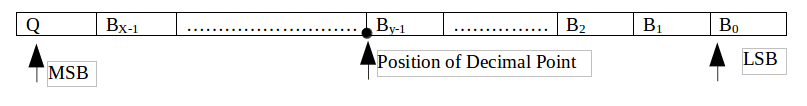
\includegraphics[scale=0.55]{figures/fpformat.png}
\caption{Fixed Point Number Representation}
\label{fig:Fixed Representation}
\end{figure}
For a given QX.Y format integer of length $(X+Y)$ bits with Y bits representing the fractional part length, the range is given by 
$[(-2^{(X-1)}),(2^{(X-1)}-2^{-Y})]$ if the integer is signed and the range is given as $[0,(2^{X}-2^{-Y})]$ if the integer is unsigned. The smallest number that can be represented in fixed point representation with fractional part length N is given as $1/N$.

\vspace{0.25cm}
While implementing in FPGA we can customize the number of bits used to represent the fractional part and integer part e.g. we can opt for 18 bits as most of the FPGA's have $18\times 18$ bit inbuilt multipliers. However the larger the number of bits used for integer and fractional part representation, the lesser is the bit error rate but at the same time the silicon area required for the design is large.

\subsection{Fixed Point Operations} \label{2.5.3}
\subsubsection{Conversion}
\textbf{Conversion from Floating Point  to Fixed  Point Format:}
Considering a floating point number A, the corresponding fixed point variable A(QX.F) can be calculated as:

\hspace{3cm}$A(QX.F)=A\times 2^{F}$,

\noindent where F represents the number of bits after the decimal or binary point.

\noindent \textbf{Conversion from Fixed Point  to Floating  Point Format:}
Given a number $A(QX.F)$ in fixed point Q format, its floating point equivalent can be calculated as:

\hspace{3cm}$A=A(QX.F)\times 2^{-F}$,

\noindent where F represents the number of bits after the decimal or binary point.


\subsubsection{Addition}
Addition operation on fractions requires the decimal values of the operands to be aligned. As seen from hardware point of view, lining up decimal points is a wire alignment step. Therefore bit shifting is needed for one or more numbers. But this leads to a loss in precision for one or more operand as the operand with higher fractional bits will be more precise. 

\vspace{0.25cm}
\noindent For two numbers having the same Q format: N1(QX.Y) and N2(QX.Y), the addition can be computed as:

\hspace{3cm}
$N1(QX.Y)+N2(QX.Y)= N3(QX.Y)$

\noindent The result is converted back to real format by performing division by a factor of $2^{Y}$.

\vspace{0.25cm}
\noindent For two numbers with different Q format: N1(QX1.Y1) and N2(QX2.Y2), the addition can be computed by first adjusting the decimal point by scaling either one number up or other number down followed by performing addition operation and scaling the result back to any required format.

\vspace{0.25cm}
\noindent e.g. Given two floating point numbers $A=2$ and $B=0.375$

\noindent Conversion of real numbers to Q4.3 format is given as:

\noindent $A(Q4.3)=2\times 2^{3} = 16$

\noindent $B(Q4.3)=0.375\times 2^{3}=3$

\noindent Computation of addition operation in fixed point Q4.3 format is given as:

\noindent $C(Q4.3)= A(Q4.3)+B(Q4.3)= 19$

\noindent Conversion of the result back, to real number is given as:

\noindent $C=C(Q4.3)/2^{3}=2.375$

\vspace{0.25cm}
\noindent In case of successive additions in the fixed point format, we can reuse the result obtained in one operation, without the need of scaling the result back after each operation. The correctness of results depends on the chosen Q format. The issues involved are loss in precision and overflow.

\vspace{.25cm}
\noindent \textbf{Overflow:} e.g. Given two floating point numbers $A=2$ and $B=0.375$

\noindent Computation of addition in fixed point Q4.3 format is given as:

\noindent $A(Q4.3)=14\times 2^{3}= 112$

\noindent $B(Q4.3)= 2.125\times 2^{3}= 17$

\noindent $C(Q4.3)= A(Q4.3)+B(Q4.3)= 129$

\noindent In the above computation, an overflow occurs and result falls out of range of an 8 bit signed integer i.e.(-128,127).

\vspace{.25cm}
\noindent \textbf{Precision:} If the above addition is performed using Q5.2 format,

\noindent $A(Q5.2)=14\times 2^{2}= 56 $

\noindent $B(Q5.2)= 2.125\times 2^{2}= 8.5$

\noindent The nearest integers to B(Q5.2) are 8 and 9 which on real number conversion generate either a value 2 or 2.25, hence B cannot be mapped directly to its original value without any precision loss.

\vspace{.25cm}
\noindent As deduced from above,the Q format used directly affects the accuracy in terms of precision loss and overflow, so the format should be carefully chosen while performing any operations on fixed point data.

\subsubsection{Multiplication}
For two numbers having the same Q format, N1(QX.Y) and N2(QX.Y) the multiplication can be computed as,


$N1(QX.Y)+N2(QX.Y)= N3(Q(1+2X).(2Y))$.

\noindent An extra scaling step is needed to convert the result back to original format.

\vspace{.25cm}
\noindent For two numbers with different Q format:N1(QX1.Y1) and N2(QX2.Y2) the multiplication can be computed as,

$N1(QX1.Y1)+N2(QX2.Y2)= N3(Q(1+X1+X2).(Y1+Y2))$

\noindent The result can be bit shifted to convert to any desired format.

\vspace{0.25cm}
\noindent e.g. Given two floating point numbers $A=2$ and $B=0.375$, computation of multiplication operation in fixed point Q4.3 format is given as:

\noindent $A(Q4.3)= 2\times 2^{3}= 16$

\noindent $B(Q4.3)= 0.375\times 2^{3}=3$

\noindent $C(Q7.6)= A(Q4.3)\times B(Q4.3)=48$

\noindent Conversion of result to floating point representation requires scaling by a factor of $2^{-6}$ instead of $2^{-3}$, therefore C can be computed as $C= C(Q7.6)/2^{6}= 0.75$.

\subsubsection{MAC}
Mostly fixed point arithmetic is used in DSP operations, which generally compute multiply accumulation operation.

\vspace{0.25cm}
\noindent Considering three real numbers $A=2$, $B=0.375$, $C=0.625$, to compute $D=A\times B+C$ in Q4.3 format. First conversion from float to fixed Q4.3 format is calculated as given below:

\noindent $A(Q4.3)=2\times 2^{3}=16$

\noindent $B(Q4.3)= 0.375\times 2^{3}=3$

\noindent $C(Q4.3)= 0.625\times 2^{3}=5$

\noindent then MAC operation is performed which is given as:

\noindent $D(Q7.6)= A(Q4.3)\times B(Q4.3)+C(Q4.3)= 16\times 3+5= 53$

\vspace{0.25cm}
\noindent In the above operation,the result of addition operation is directly used for multiplication without converting it back to real format. However in the final step, scaling is performed to get the result in floating point as given below:

\noindent $D= D(Q7.6)/2^{6}= 1.375$.

\vspace{0.25cm}
C scripts were written based on the above fixed point mathematics, for implementing the conversion, addition and multiplication operation in fixed point for analyzing the arithmetic of deep neural network which is described in chapter \ref{Chapter5}. 